% Options for packages loaded elsewhere
\PassOptionsToPackage{unicode}{hyperref}
\PassOptionsToPackage{hyphens}{url}
%
\documentclass[
]{article}
\title{Data Exploration}
\author{Team 5}
\date{15 March 2022}

\usepackage{amsmath,amssymb}
\usepackage{lmodern}
\usepackage{iftex}
\ifPDFTeX
  \usepackage[T1]{fontenc}
  \usepackage[utf8]{inputenc}
  \usepackage{textcomp} % provide euro and other symbols
\else % if luatex or xetex
  \usepackage{unicode-math}
  \defaultfontfeatures{Scale=MatchLowercase}
  \defaultfontfeatures[\rmfamily]{Ligatures=TeX,Scale=1}
\fi
% Use upquote if available, for straight quotes in verbatim environments
\IfFileExists{upquote.sty}{\usepackage{upquote}}{}
\IfFileExists{microtype.sty}{% use microtype if available
  \usepackage[]{microtype}
  \UseMicrotypeSet[protrusion]{basicmath} % disable protrusion for tt fonts
}{}
\makeatletter
\@ifundefined{KOMAClassName}{% if non-KOMA class
  \IfFileExists{parskip.sty}{%
    \usepackage{parskip}
  }{% else
    \setlength{\parindent}{0pt}
    \setlength{\parskip}{6pt plus 2pt minus 1pt}}
}{% if KOMA class
  \KOMAoptions{parskip=half}}
\makeatother
\usepackage{xcolor}
\IfFileExists{xurl.sty}{\usepackage{xurl}}{} % add URL line breaks if available
\IfFileExists{bookmark.sty}{\usepackage{bookmark}}{\usepackage{hyperref}}
\hypersetup{
  pdftitle={Data Exploration},
  pdfauthor={Team 5},
  hidelinks,
  pdfcreator={LaTeX via pandoc}}
\urlstyle{same} % disable monospaced font for URLs
\usepackage[margin=1in]{geometry}
\usepackage{graphicx}
\makeatletter
\def\maxwidth{\ifdim\Gin@nat@width>\linewidth\linewidth\else\Gin@nat@width\fi}
\def\maxheight{\ifdim\Gin@nat@height>\textheight\textheight\else\Gin@nat@height\fi}
\makeatother
% Scale images if necessary, so that they will not overflow the page
% margins by default, and it is still possible to overwrite the defaults
% using explicit options in \includegraphics[width, height, ...]{}
\setkeys{Gin}{width=\maxwidth,height=\maxheight,keepaspectratio}
% Set default figure placement to htbp
\makeatletter
\def\fps@figure{htbp}
\makeatother
\setlength{\emergencystretch}{3em} % prevent overfull lines
\providecommand{\tightlist}{%
  \setlength{\itemsep}{0pt}\setlength{\parskip}{0pt}}
\setcounter{secnumdepth}{-\maxdimen} % remove section numbering
\usepackage{booktabs}
\usepackage{longtable}
\usepackage{array}
\usepackage{multirow}
\usepackage{wrapfig}
\usepackage{float}
\usepackage{colortbl}
\usepackage{pdflscape}
\usepackage{tabu}
\usepackage{threeparttable}
\usepackage{threeparttablex}
\usepackage[normalem]{ulem}
\usepackage{makecell}
\usepackage{xcolor}
\ifLuaTeX
  \usepackage{selnolig}  % disable illegal ligatures
\fi

\begin{document}
\maketitle

\hypertarget{overview-of-the-airbnb-listings}{%
\subsubsection{Overview of the Airbnb
listings}\label{overview-of-the-airbnb-listings}}

The \texttt{combined\_data} contains listings of 17 analyzed European
cities. It captures around 200,000 observations in total, and not every
city has the same number of listings as one another. Below is an
overview of the first few rows and columns of the
\texttt{combined\_data}

\begin{table}

\caption{\label{tab:load_dataset_as_table}Table 1: Combined dataset of Airbnb listings of 16 cities}
\centering
\begin{tabular}[t]{c|c|c|c|c|c|c|c}
\hline
id & name & room\_type & price & min\_nights & reviews & city & country\\
\hline
15883 & b\&b near Old Danube river & Hotel room & 120 & 1 & 14 & vienna & AUT\\
\hline
38768 & central cityapartement- wifi- nice neighbourhood & Entire home/apt & 66 & 3 & 336 & vienna & AUT\\
\hline
40625 & Near Palace Schönbrunn, Apt. 1 & Entire home/apt & 156 & 1 & 162 & vienna & AUT\\
\hline
51287 & little studio- next to citycenter- wifi- nice area & Entire home/apt & 62 & 3 & 327 & vienna & AUT\\
\hline
70637 & Flat in the Center with Terrace & Private room & 50 & 2 & 117 & vienna & AUT\\
\hline
75471 & nice big apartment with balcony & Entire home/apt & 77 & 3 & 50 & vienna & AUT\\
\hline
75500 & Lovely Viennese apartment (2-4 p.) & Entire home/apt & 65 & 4 & 14 & vienna & AUT\\
\hline
90247 & Beautiful New Central Apartment & Entire home/apt & 98 & 1 & 631 & vienna & AUT\\
\hline
109679 & Near Palace Schönbrunn, Apt. 4 & Entire home/apt & 101 & 1 & 123 & vienna & AUT\\
\hline
111059 & Modern Apartment, 10min to the City & Entire home/apt & 52 & 3 & 152 & vienna & AUT\\
\hline
\end{tabular}
\end{table}

After loading the dataset, we can start with inspection of ``typical
value'' and ``location'' for each variable.

\hypertarget{estimates-of-location}{%
\subsubsection{Estimates of location}\label{estimates-of-location}}

\begin{table}
\centering
\begin{tabular}[t]{lllllllllllllllllll}
\toprule
  & amsterdam & antwerp & barcelona & berlin & brussels & copenhagen & london & madrid & manchester & munich & prague & rome & thessaloniki & valencia & vaud & venice & vienna & Overall\\
\midrule
 & (N=5556) & (N=1749) & (N=15707) & (N=17290) & (N=5249) & (N=9726) & (N=66641) & (N=17831) & (N=3447) & (N=4995) & (N=6782) & (N=24627) & (N=2548) & (N=5546) & (N=4634) & (N=7352) & (N=11429) & (N=211109)\\
\addlinespace[0.3em]
\multicolumn{19}{l}{\textbf{Room Types}}\\
\hspace{1em}Entire home/apt & 3701 (66.6\%) & 1379 (78.8\%) & 8407 (53.5\%) & 9844 (56.9\%) & 3724 (70.9\%) & 8343 (85.8\%) & 37472 (56.2\%) & 10846 (60.8\%) & 2030 (58.9\%) & 3014 (60.3\%) & 5196 (76.6\%) & 15874 (64.5\%) & 2439 (95.7\%) & 3829 (69.0\%) & 3234 (69.8\%) & 5665 (77.1\%) & 8591 (75.2\%) & 133588 (63.3\%)\\
\hspace{1em}Hotel room & 87 (1.6\%) & 10 (0.6\%) & 220 (1.4\%) & 165 (1.0\%) & 49 (0.9\%) & 24 (0.2\%) & 257 (0.4\%) & 153 (0.9\%) & 18 (0.5\%) & 56 (1.1\%) & 236 (3.5\%) & 964 (3.9\%) & 5 (0.2\%) & 24 (0.4\%) & 35 (0.8\%) & 207 (2.8\%) & 64 (0.6\%) & 2574 (1.2\%)\\
\hspace{1em}Private room & 1747 (31.4\%) & 354 (20.2\%) & 6858 (43.7\%) & 7072 (40.9\%) & 1434 (27.3\%) & 1340 (13.8\%) & 28402 (42.6\%) & 6594 (37.0\%) & 1380 (40.0\%) & 1858 (37.2\%) & 1255 (18.5\%) & 7650 (31.1\%) & 101 (4.0\%) & 1672 (30.1\%) & 1341 (28.9\%) & 1450 (19.7\%) & 2694 (23.6\%) & 73202 (34.7\%)\\
\hspace{1em}Shared room & 21 (0.4\%) & 6 (0.3\%) & 222 (1.4\%) & 209 (1.2\%) & 42 (0.8\%) & 19 (0.2\%) & 510 (0.8\%) & 238 (1.3\%) & 19 (0.6\%) & 67 (1.3\%) & 95 (1.4\%) & 139 (0.6\%) & 3 (0.1\%) & 21 (0.4\%) & 24 (0.5\%) & 30 (0.4\%) & 80 (0.7\%) & 1745 (0.8\%)\\
\addlinespace[0.3em]
\multicolumn{19}{l}{\textbf{Price per night}}\\
\hspace{1em}Mean (SD) & 168 (167) & 110 (184) & 98.9 (218) & 75.3 (141) & 91.8 (127) & 1120 (2250) & 145 (350) & 135 (382) & 164 (317) & 128 (374) & 9020 (128000) & 128 (483) & 62.3 (60.7) & 83.5 (165) & 153 (330) & 207 (1070) & 83.1 (185) & 459 (23000)\\
\hspace{1em}Median [Min, Max] & 139 [0, 6480] & 78.0 [13.0, 5800] & 68.0 [0, 10000] & 55.0 [0, 11000] & 69.0 [0, 3500] & 875 [0, 100000] & 83.0 [0, 18600] & 72.0 [0, 16000] & 80.0 [10.0, 7370] & 81.0 [0, 10000] & 1710 [0, 2870000] & 75.0 [0, 21000] & 50.0 [9.00, 1510] & 64.0 [9.00, 8000] & 93.0 [9.00, 9200] & 100 [0, 16800] & 60.0 [0, 10000] & 80.0 [0, 2870000]\\
\addlinespace[0.3em]
\multicolumn{19}{l}{\textbf{Minimum nights}}\\
\hspace{1em}Mean (SD) & 3.58 (20.0) & 5.16 (21.4) & 14.4 (36.1) & 10.4 (36.4) & 10.1 (35.1) & 4.77 (21.2) & 6.65 (30.4) & 7.43 (36.6) & 9.47 (43.8) & 9.01 (31.4) & 5.46 (40.3) & 3.60 (18.1) & 3.51 (18.0) & 6.18 (28.0) & 7.71 (101) & 2.46 (8.46) & 5.95 (24.3) & 7.01 (33.4)\\
\hspace{1em}Median [Min, Max] & 2.00 [1.00, 1000] & 2.00 [1.00, 500] & 3.00 [1.00, 1120] & 3.00 [1.00, 1120] & 2.00 [1.00, 1130] & 3.00 [1.00, 1110] & 2.00 [1.00, 1130] & 2.00 [1.00, 1130] & 2.00 [1.00, 365] & 2.00 [1.00, 1000] & 2.00 [1.00, 1000] & 2.00 [1.00, 1000] & 2.00 [1.00, 365] & 2.00 [1.00, 1000] & 2.00 [1.00, 6670] & 2.00 [1.00, 400] & 2.00 [1.00, 1130] & 2.00 [1.00, 6670]\\
\addlinespace[0.3em]
\multicolumn{19}{l}{\textbf{Number of reviews}}\\
\hspace{1em}Mean (SD) & 49.0 (89.1) & 36.0 (62.0) & 35.8 (69.3) & 23.9 (53.4) & 37.0 (71.8) & 20.4 (37.4) & 15.7 (36.8) & 36.1 (68.9) & 31.4 (61.7) & 22.3 (55.7) & 54.9 (85.1) & 42.9 (72.8) & 39.9 (63.4) & 41.3 (65.3) & 16.2 (31.8) & 64.2 (92.8) & 31.9 (61.2) & 29.8 (60.8)\\
\hspace{1em}Median [Min, Max] & 17.0 [0, 901] & 13.0 [0, 648] & 5.00 [0, 883] & 5.00 [0, 916] & 10.0 [0, 797] & 8.00 [0, 676] & 3.00 [0, 974] & 7.00 [0, 767] & 9.00 [0, 1300] & 4.00 [0, 765] & 17.0 [0, 928] & 10.0 [0, 829] & 16.0 [0, 574] & 13.0 [0, 678] & 4.00 [0, 460] & 25.0 [0, 765] & 7.00 [0, 632] & 6.00 [0, 1300]\\
\addlinespace[0.3em]
\multicolumn{19}{l}{\textbf{Availability}}\\
\hspace{1em}Mean (SD) & 106 (129) & 195 (139) & 175 (138) & 86.5 (128) & 165 (134) & 98.2 (127) & 99.7 (134) & 148 (140) & 197 (132) & 135 (136) & 176 (137) & 210 (134) & 233 (128) & 175 (128) & 149 (140) & 224 (130) & 143 (144) & 140 (142)\\
\hspace{1em}Median [Min, Max] & 34.0 [0, 365] & 182 [0, 365] & 179 [0, 365] & 0 [0, 365] & 153 [0, 365] & 28.0 [0, 365] & 2.00 [0, 365] & 104 [0, 365] & 178 [0, 365] & 88.0 [0, 365] & 166 [0, 365] & 249 [0, 365] & 281 [0, 365] & 168 [0, 365] & 118 [0, 365] & 270 [0, 365] & 90.0 [0, 365] & 88.0 [0, 365]\\
\addlinespace[0.3em]
\multicolumn{19}{l}{\textbf{New reviews received}}\\
\hspace{1em}Mean (SD) & 6.06 (17.8) & 9.44 (15.1) & 5.13 (11.5) & 3.61 (13.2) & 7.26 (13.8) & 3.18 (6.97) & 2.08 (7.47) & 6.52 (13.3) & 9.54 (17.1) & 3.49 (12.7) & 7.58 (15.4) & 4.93 (10.1) & 9.86 (14.4) & 8.83 (12.2) & 4.68 (9.38) & 8.49 (14.2) & 4.96 (11.0) & 4.52 (11.4)\\
\hspace{1em}Median [Min, Max] & 1.00 [0, 597] & 3.00 [0, 143] & 0 [0, 460] & 0 [0, 658] & 2.00 [0, 172] & 1.00 [0, 235] & 0 [0, 516] & 1.00 [0, 347] & 4.00 [0, 472] & 0 [0, 450] & 1.00 [0, 626] & 0 [0, 476] & 4.00 [0, 112] & 4.00 [0, 164] & 0 [0, 110] & 2.00 [0, 444] & 0 [0, 396] & 0 [0, 658]\\
\bottomrule
\end{tabular}
\end{table}

According to the statistics summary, entire home/apartment accumulates
more than half of the observations. This tendency also appears across
listings of each city. Taking up the second most offered type of room is
private room. What we could take on from here is that the Airbnb
landscape in European market values privacy and personal comfort but at
the same time the guests can stay close to local neighbourhood compared
to traditional hotels.

\begin{center}\includegraphics{data_exploration_files/figure-latex/distribution of price as a whole-1} \end{center}

In terms of price, we have noticed different variation in price range,
which is caused by how each listing is scraped in local currency. It
could also be misled by the outliers of expensive entire home/apartment.
Particularly, an average night price staying in Prague is 9020 Kč (≈ 360
€) and could vary up to maximum 2870000, whereas one night in London
costs on average 145 £ (≈ 172 €). Furthermore, when looking at the
measure of spread, most of price observations in Prague listing fall
within above/below 128,000 Kč, indicating a wide data dispersion around
the average price. Therefore, plotting distribution of Airbnb price as a
whole can give us a false sense of description of location and data
spread.

\begin{center}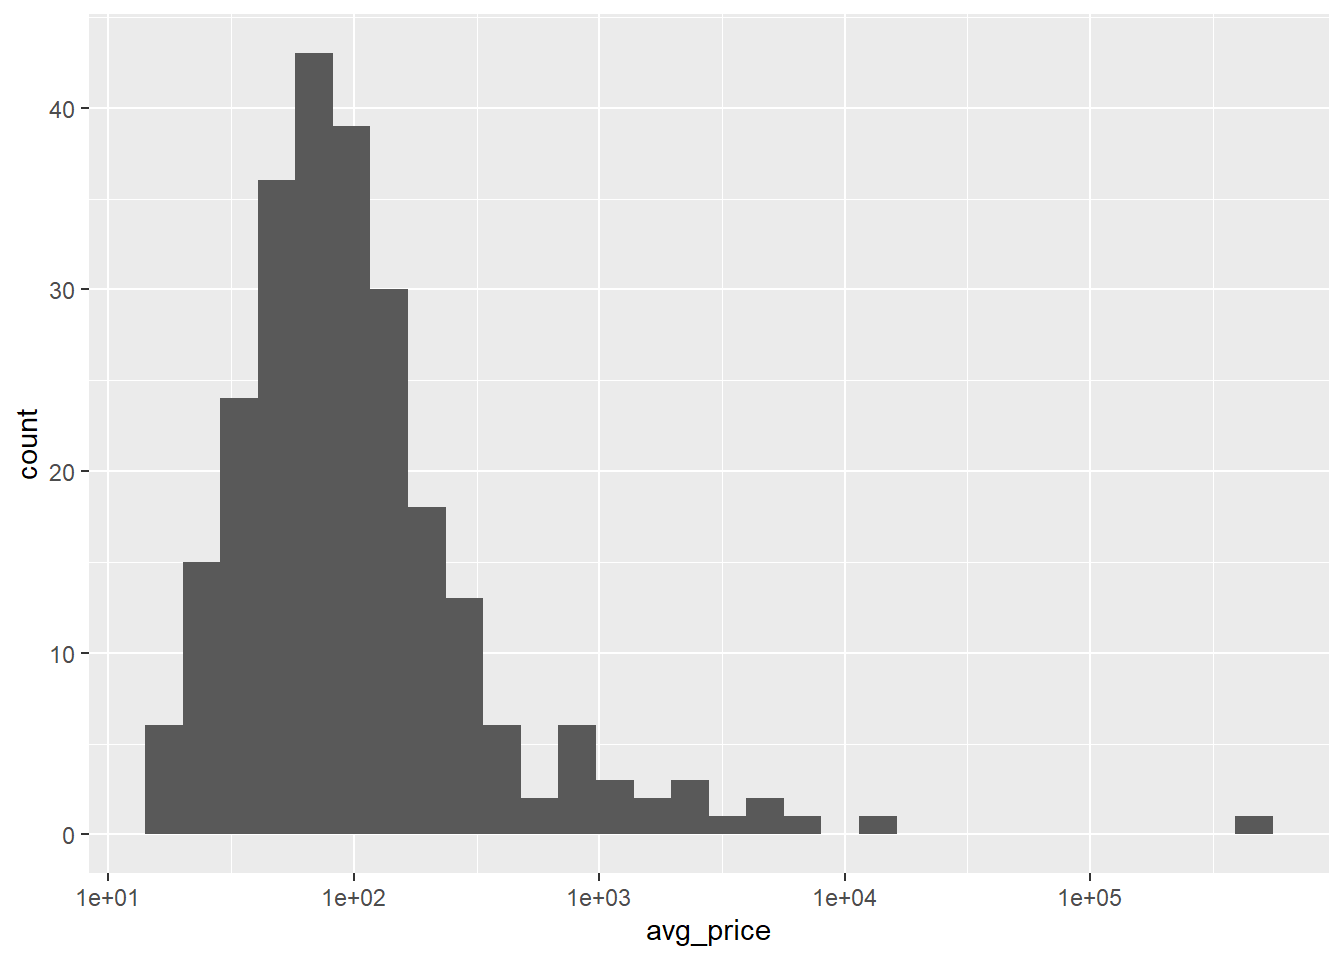
\includegraphics{data_exploration_files/figure-latex/distribution of price by country-1} \end{center}

Without taking the log transformation to cancel out different units of
measurement, we may assert a counter-intuitive conclusion, implying
Prague is least affordable city for holiday than London. In fact, cities
like Amsterdam and London are one of the top expensive destinations
(Statista, 2021). Besides, logarithm of price is a basic yet effective
approach to deal with non-normal distributed data.

\hypertarget{references}{%
\subsubsection{References}\label{references}}

Statista. (2021). Least affordable cities for backpacking in Europe for
2020, by daily price index (in U.S. dollars). Retrieved from
\url{https://www.statista.com/statistics/696870/most-expensive-cities-for-backpacking-europe/}

Statista. (2021). Cheapest cities to visit in Europe as of December
2021, by daily price. Retrieved from
\url{https://www.statista.com/statistics/696725/most-affordable-cities-for-backpacking-europe/}

\end{document}
